\documentclass[18pt, spanish]{beamer}


\usetheme{Warsaw}
\usepackage[utf8]{inputenc}
\usepackage{amsmath}
%\usepackage{amsfonts}
\usepackage{amssymb}
\usepackage{graphicx}
%\usepackage{alltt} %para permitir usar el comando \verb
% Para trabajar en idioma español
\usepackage[T1]{fontenc}
\usepackage{selinput}
\SelectInputMappings{%
  aacute={á},
  ntilde={ñ},
  Euro={€}
}
\usepackage{babel}
%%%%%%%%%%%%
\author{Ing. Cristian Montero}
\title{Introducción a \LaTeX}
%\setbeamercovered{transparent} 
%\setbeamertemplate{navigation symbols}{} 
%\logo{} 
\institute{ResBaz 2016} 
\date{} 
%\subject{} 

\begin{document}

\begin{frame}
\titlepage
\end{frame}

\begin{frame}{Contenidos}
\tableofcontents
\end{frame}

\section{Introducción}
\subsection{Qué es \LaTeX?}
\begin{frame}{•}
\frametitle{Qué es \LaTeX?}
\begin{itemize}
	\item Es un sistema Open source de preparacion de documentos.
	\item Escrito por Leslie Lamport bassado en TeX de Donald Knuth \footnote{http://www.tug.org/whatis.html}
	\item Utiliza un lenguaje de marcado similar a HTML
	
\end{itemize}
\end{frame}

\subsection{Beneficios}
\begin{frame}
\frametitle{Beneficios}
\begin{itemize}
	\item Adecuado para documentos técnicos y científicos.
	\item Evita el lidiar demasiado con el formato del documento.	
	\item Capacidades de citado y referenciado.
	\item Generacion automatica de listas de contenidos, figuras y tablas, indices glosarios y bibliografia.
	\item Multi-lenguaje
	\item Pantillas para cartas, presentaciones, contables, libros, etc.
	\item Gran variedad de extensiones disponibles
	\item Portable (Multiplataforma)
\end{itemize}
\end{frame}

\subsection{Procesadores de texto}
\begin{frame}
\frametitle{Que pasa con los procesadores de texto?}
\begin{itemize}
	\item Contienen comandos de formato escondidos.
	\item Virus podrian adherirse a los archivos.
	\item Problemas de compatibilidad incluso entre versiones.
\end{itemize}

\end{frame}

\section{Ejercicios}

\begin{frame}[fragile]
\frametitle{Hola mundo!}
\begin{verbatim}

\documentclass{article}
\begin{document}
	Hola Mundo.
\end{document}

\end{verbatim}
\end{frame}


\begin{frame}[fragile]
\frametitle{Agregando titulos}
\begin{verbatim}
\documentclass[a4paper,11pt, spanish]{article}
\begin{document}
\title{Ejemplo 2}
\author{Nombre del autor}
\date{Febrero 14, 2015}
\maketitle
\section{Qué es esto?}
Este es nuestro segundo documento.

Este incluye información adicional.
\end{document}
\end{verbatim}

\end{frame}

\begin{frame}[fragile]
\frametitle{Caracteres especiales}
\begin{verbatim}

\documentclass{article}
\begin{document}
Statement \#1:
50\% of \$100 makes \$50.
More special symbols are \&, \_, \{ and \}.
\end{document}

\end{verbatim}
\end{frame}


\begin{frame}[fragile]
\frametitle{Dando Formato}
\begin{verbatim}

\documentclass{article}
\begin{document}
Text can be \emph{emphasized}.
Besides being \textit{italic} words could be \textbf{bold},
\textsl{slanted} or typeset in \textsc{Small Caps}.
Such commands can be \textit{\textbf{nested}}.
\emph{See how \emph{emphasizing} looks when nested.}
\end{document}

\end{verbatim}
\end{frame}

\begin{frame}[fragile]
\frametitle{Dando Formato - Resumen Comandos}
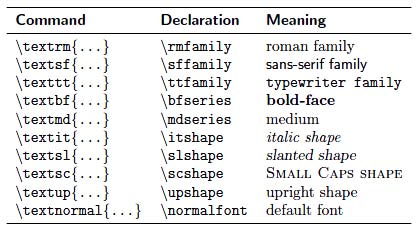
\includegraphics[scale=1]{Imagenes/formato_texto.jpg}
\end{frame}

\begin{frame}[fragile]
\frametitle{Incluyendo Citas}
\begin{verbatim}
\documentclass{article}
\begin{document}
Niels Bohr said: "An expert is a person who has made
all the mistakes that can be made in a very narrow field.''
Albert Einstein said:
\begin{quote}
Anyone who has never made a mistake has never tried anything new.
\end{quote}
Errors are inevitable. So, let's be brave trying something new.
\end{document}
\end{verbatim}
\end{frame}


\begin{frame}[fragile]
\frametitle{Estructura de un artículo}
\begin{itemize}
	\item Encabezado (Título, autor, fecha)
	\item Resumen (Abstract)
	\item Sección
	\item Subsecciones
	\item Sub subsecciones	
\end{itemize}
Ver archivo Ejercicio 6.
\end{frame}

\section{Gráficos, tablas y fórmulas}
\begin{frame}[fragile]
\frametitle{Gráficos}
\begin{itemize}
	\item Se debe incluir la librería \textbf{graphix} 
\end{itemize}
\begin{verbatim}
	\usepackage{graphicx}
\end{verbatim}
\begin{itemize}
	\item Utilizar el siguiente código para incluir la imagen.
	\item Utilizar de preferencia imágenes png, pdf, eps.
\end{itemize}
\begin{verbatim}

\begin{figure}[p]
    \centering
    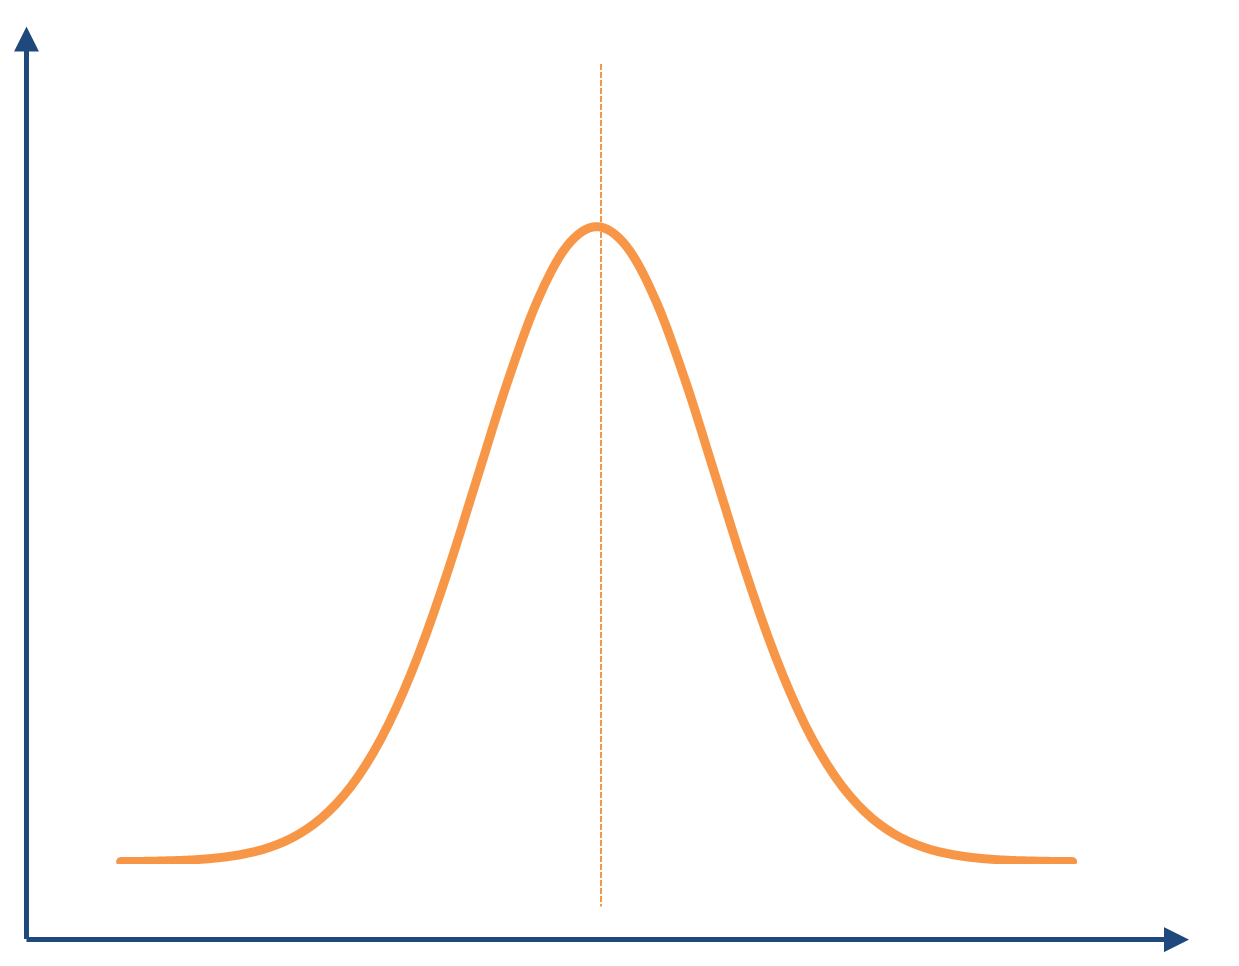
\includegraphics[width=0.3]{BellCurve.png}
    \caption{Awesome Image}
    \label{fig:bell_curve}
\end{figure}

\end{verbatim}
\end{frame}

\begin{frame}[fragile]
\frametitle{Tablas}

\begin{itemize}
	\item Alineación del texto  
	\begin{description}
		\item[l] Columna alineada a la izquierda
		\item[c] Columna alineada al centro
		\item[r] Columna alineada a la derecha
		\item[p\{anchura\}] Columna con ancho definido con texto justificado
	\end{description}
	\item Opciones adicionales
	\begin{description}
		\item[$|$ (pipe)] Línea vertical
		\item[$||$] Doble línea vertical
		\item[\&] Separador de Columna
		\item[]\verb|\\| Inicio nueva linea
		\item[]\verb;\hline; Linea horizontal
	\end{description}
		 
\end{itemize}
\end{frame}

\begin{frame}[fragile]
\frametitle{Tablas}
\begin{verbatim}
	\begin{table}[h]
		\centering
		\begin{tabular}{| c || l |}
	    	\hline \hline
	     	No. & Nombre \\
     		\hline \hline
      		1 & Lunes \\
      		2 & Martes \\
	      	3 & Miércoles \\
    	  	4 & Jueves \\
      		5 & Viernes \\
	      	6 & Sábado \\
    	  	7 & Domingo \\
      		\hline
		  \end{tabular}
  		\caption{Días de la semana}
	\end{table}
\end{verbatim}
\end{frame}


\begin{frame}[fragile]
\frametitle{Fórmulas}
\begin{itemize}
	\item Se debe incluir la librería \textbf{asmath} o\textbf{mathtools} 
\end{itemize}
\begin{verbatim}
	\usepackage{asmath}
\end{verbatim}
\begin{itemize}
	\item Extensa lista de símbolos para ser utilizados
	\item \url{https://en.wikibooks.org/wiki/LaTeX/Mathematics}
\end{itemize}
Fórmula de ejemplo:
\begin{verbatim}

$ \lim_{x \to \infty} \exp(-x) = 0 $

			\begin{equation} \label{eq:2}
			P\left(A=2\middle|\frac{A^2}{B}>4\right)
			\end{equation}

\end{verbatim}
\end{frame}

\begin{frame}[allowframebreaks]{Referencias}
\raggedright
\nocite{*}
\bibliographystyle{plain}
\bibliography{references}
\end{frame}

\end{document}